\documentclass[fleqn]{article}
\usepackage[margin=1.5cm]{geometry}   % shrink margins

\usepackage{amsmath}    % math equation environments
\usepackage{amssymb}    % math symbols such as natural numbers N.

\usepackage{multicol}	% can be used to put enumerate in columns. Usage: \begin{multicols}{NumCols}\begin{enumerate}...

\newcommand\Item[1][]{ % custom \Item command for block math
  \ifx\relax#1\relax  \item \else \item[#1] \fi
  \abovedisplayskip=0pt\abovedisplayshortskip=0pt~\vspace*{-\baselineskip}
}

\newcommand*{\perm}[2]{{}^{#1}\!P_{#2}}%
\newcommand*{\comb}[2]{{}^{#1}C_{#2}}%

\usepackage{tikz}	% for diagrams
\usetikzlibrary{positioning}

% \usepackage{adjustbox}	% align enumerations containing tall objects to top. Usage: \item\adjustbox{valign=t}{...}

% \usepackage{centernot}	% centers not symbol. Usage: \centernot{...}

% Math mode in tables. Usage: use column type C
% \usepackage{array}   % for \newcolumntype macro
% \newcolumntype{C}{>{$}c<{$}} % math-mode version of "c" column type

% paragraph indentation within enumerations
\usepackage{enumitem}
\setlist{parsep=4pt,listparindent=\parindent}

\title{Discrete Mathematics \\
\large Homework 7}
\author{Abraham Murciano}

\begin{document}

\maketitle

\begin{enumerate}

    \item[4.]
    \begin{enumerate}
		\item % a
		\begin{multicols}{2}
			\begin{enumerate}
				\Item \[4! \times 4! = 576\]
				\Item \[4! \times 4! \times 2 = 1152\]
				\Item \[4! \times 4! \times 2 = 1152\]
				\Item \[8! = 40320\]
			\end{enumerate}
		\end{multicols}
		\item % b
		\begin{multicols}{2}
			\begin{enumerate}
				\Item \[5! \times 4! \times 3! \times 3! = 103,680\]
				\Item \[5! \times 4! \times 5! = 345,600\]
				\Item \[5! \times 4! \times 4! = 69,120 \]
				\Item \[12! = 479,001,600 \]
			\end{enumerate}
		\end{multicols}
	\end{enumerate}

	\bigskip
	\item[6.]
	\begin{multicols}{3}
		\begin{enumerate}
			\Item \[\comb{12}{4} = 495\]
			\Item \[\comb{3}{1} \times \comb{9}{3} = 252\]
			\Item \[\comb{12}{4} - \comb{9}{4} = 369\]
		\end{enumerate}
	\end{multicols}

	\bigskip
	\item [24.]
	Twenty men can be split into four teams of five players each in \(\begin{aligned}\binom{20}{5, 5, 5, 5}\end{aligned}\) ways. This is equal to 11,732,745,024.

	\bigskip
	\item[25.]
	\begin{multicols}{2}
		\begin{enumerate}
			\Item \[\binom{4 + 7 - 1}{7} = 120\]
			\Item \[7^4 = 2401\]
		\end{enumerate}
	\end{multicols}
	
	\bigskip
	\item[26.]
	\begin{multicols}{2}
		\begin{enumerate}
			\Item \[\binom{7 + 7 - 1}{7} = 1716\]
			\Item \[\binom{7 + 10 - 1}{10} = 8008\]
		\end{enumerate}
	\end{multicols}

	\bigskip
	\item[27.]
	\begin{multicols}{2}
		\begin{enumerate}
			\Item[(b)] \[\binom{9 + 15 - 1}{15} = 490,314\]
			\Item[(c)] \[\binom{10 + 20 - 1}{20} - \binom{10 + 15 - 1}{15} = 8,707,501\]
		\end{enumerate}
	\end{multicols}
	\begin{enumerate}
		\item[(e)]
		\begin{multicols}{2}
			\begin{enumerate}
				\Item \[\binom{9 + 16 - 1}{16} = 735,471\]
				\Item \[\binom{10 + 21 - 1}{21} - \binom{10 + 16 - 1}{16} = 12,264,175\]
			\end{enumerate}
		\end{multicols}
	\end{enumerate}

	\bigskip
	\item[28.]
	\begin{multicols}{3}
		\begin{enumerate}
			\Item \[{(m + 1)}^n\]
			\Item \[m!\]
			\Item \[\comb{5}{1} \times \comb{4}{1} \times 3^3 = 540\]
		\end{enumerate}
	\end{multicols}

	\bigskip
	\item[29.]
	\begin{enumerate}
		\item[(b)] 
		There are infinitely many solutions, since there is no lower bound on the variables \(d\) and \(e\).
		\item[(d)]
		We must find the number of solutions for te following equation given that all the variables are nonnegative, and \(a, b, c\) are odd and \(d, e\) are even.
		\begin{equation*}
			a + b + c + d + e = 15
		\end{equation*}

		Due to the parity restrictions, we have the following equations, where all the variables \(x'\) are nonnegative.
		\begin{gather*}
			a = 2a' + 1 \\
			b = 2b' + 1 \\
			c = 2c' + 1 \\
			d = 2d' \\
			e = 2e'
		\end{gather*}

		We can now substitute each variable from the original equation with an equivalent value from another of the equations, to obtain
		\begin{gather*}
			2a' + 1 + 2b' + 1 + 2c' + 1 + 2d' + 2e' = 15 \\
			2a' + 2b' + 2c' + 2d' + 2e' = 18 \\
			a' + b' + c' + d' + e' = 9
		\end{gather*}

		Therefore the number of solutions is:
		\[\binom{5 + 9 - 1}{9} = 715\]
	\end{enumerate}

	\bigskip
	\item[31.]
	\begin{enumerate}
		\item % a
		\begin{enumerate}
			\Item % i
			\[\binom{3 + 30 - 1}{30} = 496\]
			\Item % ii
			\[\binom{3 + 40 - 1}{40} - \binom{3 + 29 - 1}{29} = 396\]
		\end{enumerate}
		\Item % b
		\[\binom{3 + 300 - 1}{300} - 3 \binom{3 + 120 - 1}{120} = 23,308\]
	\end{enumerate}

	\bigskip
	\item[32.]
	\begin{multicols}{2}
		\begin{enumerate}
			\Item % a
			\[4^3 = 64\]
			\Item % b
			\[\comb{4}{3} = 4\]
		\end{enumerate}
	\end{multicols}

	\bigskip
	\item[33.]
	\begin{multicols}{2}
		\begin{enumerate}
			\Item \[\binom{6 + 10 - 1}{10} = 3003\]
			\Item \[3003 - \binom{6 + 10 - 6 - 1}{4} = 2877\]
		\end{enumerate}
	\end{multicols}

	\item[36.]
	Lay the \(n\) 1's in a row. There are \(n + 1\) places where any number of 0's could be inserted; \(n - 1\) places are between two 1's, and two places are on either end of the row of 1's, as shown in figure \ref{row of 1's}.
	\begin{figure}[h]
		\centering
		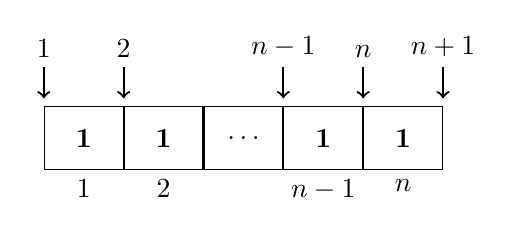
\begin{tikzpicture}[
			element/.style = {rectangle, draw=black, thin, minimum height=.8cm, minimum width=1cm}
		]
			\node[element] (1) {\textbf{1}};
			\node[element] (2) [right=0cm of 1] {\textbf{1}};
			\node[element] (3) [right=0cm of 2] {\(\dots\)};
			\node[element] (4) [right=0cm of 3] {\textbf{1}};
			\node[element] (5) [right=0cm of 4] {\textbf{1}};

			\node (pos1) [below=0cm of 1] {1};
			\node (pos2) [below=0cm of 2] {2};
			\node (pos4) [below=0cm of 4] {\(n-1\)};
			\node (pos5) [below=0cm of 5] {\(n\)};

			\node (arrow1) [above=.5cm of 1.north west] {1};
			\draw [shorten >=0.1cm, ->] [thick] (arrow1) -- (1.north west);
			\node (arrow2) [above=.5cm of 2.north west] {2};
			\draw [shorten >=0.1cm, ->] [thick] (arrow2) -- (2.north west);
			\node (arrow4) [above=.5cm of 4.north west] {\(n-1\)};
			\draw [shorten >=0.1cm, ->] [thick] (arrow4) -- (4.north west);
			\node (arrow5) [above=.5cm of 5.north west] {\(n\)};
			\draw [shorten >=0.1cm, ->] [thick] (arrow5) -- (5.north west);
			\node (arrow6) [above=.5cm of 5.north east] {\(n+1\)};
			\draw [shorten >=0.1cm, ->] [thick] (arrow6) -- (5.north east);
		\end{tikzpicture}
		\caption{Row of \(n\) 1's with \(n + 1\) spaces to insert 0's}
		\label{row of 1's}
	\end{figure}

	However, since no two 1's may be adjacent, there must be at least one 0 in all the spots 2 through \(n\). Now that we have accounted for the positions of \(n - 1\) of the 0's, there are \(m - (n - 1) = m - n + 1\) remaining 0's to place, with \(n + 1\) positions to place them. This gives us the number of ways to arrange \(n\) 1's and \(m\) 0's with no two 1's being adjacent to be equal to:
	\[\binom{(n + 1) + (m - n + 1) - 1}{m - n + 1} = \binom{m + 1}{m - n + 1} = \binom{m + 1}{(m + 1) - (m - n + 1)} = \binom{m + 1}{n}\]

\end{enumerate}
    
\end{document}
